\documentclass[letterpaper]{article} % DO NOT CHANGE THIS
\usepackage[submission]{aaai2027}  % DO NOT CHANGE THIS
% The serif, sans-serif, and monospaced fonts are loaded automatically by
% aaai2027.sty (newtxtext, helvet, courier). DO NOT add \usepackage{times},
% \usepackage{helvet}, \usepackage{courier}, or any other font package.
\usepackage[hyphens]{url}  % DO NOT CHANGE THIS
\usepackage{graphicx} % DO NOT CHANGE THIS
\urlstyle{rm} % DO NOT CHANGE THIS
\def\UrlFont{\rm}  % DO NOT CHANGE THIS
\usepackage{natbib}  % DO NOT CHANGE THIS AND DO NOT ADD ANY OPTIONS TO IT
\usepackage{caption} % DO NOT CHANGE THIS AND DO NOT ADD ANY OPTIONS TO IT
\frenchspacing  % DO NOT CHANGE THIS
%
% These are recommended to typeset algorithms but not required. See the subsubsection on algorithms. Remove them if you don't have algorithms in your paper.
\usepackage{algorithm}
\usepackage{algorithmic}
%
% These are recommended to typeset listings but not required. See the subsubsection on listing. Remove this block if you don't have listings in your paper.
\usepackage{newfloat}
\usepackage{listings}
\DeclareCaptionStyle{ruled}{labelfont=normalfont,labelsep=colon,strut=off} % DO NOT CHANGE THIS
\lstset{%
	basicstyle={\footnotesize\ttfamily},% footnotesize acceptable for monospace
	numbers=left,numberstyle=\footnotesize,xleftmargin=2em,% show line numbers, remove this entire line if you don't want the numbers.
	aboveskip=0pt,belowskip=0pt,%
	showstringspaces=false,tabsize=2,breaklines=true}
\floatstyle{ruled}
\newfloat{listing}{tb}{lst}{}
\floatname{listing}{Listing}
%
% Recommended for better-looking tables
\usepackage{booktabs}
\usepackage{amsmath}
%
% Keep the \pdfinfo as shown here. There's no need
% for you to add the /Title and /Author tags.
\pdfinfo{
/TemplateVersion (2027.1)
}

\setcounter{secnumdepth}{0}

\title{TERM: Trustworthy Embodied Robotics Modeling\\Multi-Stream Fusion and Dual Action Heads for Language-Conditioned Manipulation}
\author{Anonymous Submission}
\affiliations{}

\begin{document}

\maketitle

\begin{abstract}
What does a robot do when it misses? Most vision-language-action (VLA) policies have no answer: each action is a stateless function of the current image and task instruction, with no memory of what was just attempted or whether it worked. This is not a simplification---it is a structural barrier to recovery, adaptation, and interpretable behavior.

We present TERM (Trustworthy Embodied Robotics Modeling), a closed-loop policy that routes action history and its consequences back into the decision process through \emph{language}---the same modality used to communicate goals. By verbalizing what was last attempted and what it produced, TERM re-encodes both signals through a frozen vision-language encoder, so that prior actions and their spatial outcomes occupy a representation space already aligned with the task instruction. The result is a policy that can read its own history the same way it reads a goal.

Two design decisions distinguish TERM from prior closed-loop work. First, a bidirectional fusion transformer with full cross-stream attention is architecturally necessary: under causal masking, feedback tokens are structurally blind to the current visual scene and the closed-loop mechanism is entirely inert. Second, two action heads serve disjoint roles---one drives the robot at inference, the other provides dense geometric supervision during training and cycles its own spatial predictions back as self-knowledge, never touching inference. Systematic ablation confirms that each component earns its place, and that the gains are architectural, not a product of scale.
\end{abstract}

\section{Introduction}

Enabling robots to follow natural language instructions requires bridging a deep gap: instructions operate at the level of goal semantics (``push the star near the moon'') while motor control operates at the level of end-effector displacements. Vision-language-action models \cite{brohan2023rt2,black2024pi0,kim2024openvla} have demonstrated that large pretrained vision-language encoders can be adapted for robotic control, but a structural limitation persists across all mainstream designs: the policy is stateless at inference. Each action is a function only of the current camera frame and task instruction, discarding two highly informative signals from prior steps---what was attempted and whether it succeeded.

The consequences are predictable. A robot that fails a push action (e.g., misses the block) has no mechanism to recognize failure and adapt. The reward signal that RL training relies on is absent at deployment. Recovery behaviors, which require comparing the current observation to the expected outcome of the last action, are impossible without a memory of that expectation. Existing closed-loop designs \cite{hejna2025pi05,durante2024agent} encode prior actions numerically but carry no representation of whether those actions achieved their intended spatial effect.

We address these limitations with TERM (Trustworthy Embodied Robotics Modeling). TERM's central insight is to route action history and its consequences back through \emph{language}---the same modality used to encode task instructions. The string ``pushed the block rightward'' and the string ``I moved significantly closer to the goal and received a moderate reward'' already encode geometric and evaluative meaning in the same frozen representation space used for goal encoding. By converting the prior action and the resulting spatial outcome into natural language, TERM grounds the closed-loop signal in representations intrinsically aligned with the task instruction---without additional encoders or pretraining.

The five-stream architecture fuses vision, instruction, trustworthy safety narration ($E_{act}$), embodied knowledge planning ($E_{conseq}$), and numerical action history through a bidirectional fusion transformer with no causal mask. Bidirectional attention is architecturally essential: under causal masking, the feedback tokens appear early in the sequence and are completely blind to the current visual scene, defeating their purpose as closed-loop signals.

Two action heads decode the fused CLS representation with clearly separated roles. The \texttt{action\_bin\_head} classifies the intended motion into one of eight discrete directional bins and is the sole driver of robot motion at inference. The \texttt{action\_vec\_head} regresses a continuous 2D displacement vector $[\Delta x, \Delta y]$ that is never used at inference to drive the robot; instead, it provides geometric gradient supervision during training and cycles its prediction back into the history stream so that the model has explicit, spatially grounded knowledge of its own predicted intent at each prior step.

Our contributions are: (1) the TERM architecture combining five specialized streams and bidirectional fusion; (2) identification and correction of the causal-mask failure mode that prevents feedback tokens from attending to visual context; (3) a dual-head decoding strategy with \texttt{action\_bin\_head} for stable discrete control and \texttt{action\_vec\_head} for geometric supervision and closed-loop self-feedback; and (4) systematic ablation on Language-Table demonstrating the contribution of each component.

\section{Related Work}

\paragraph{Vision-Language-Action Models.}
RT-2 \cite{brohan2023rt2} co-fine-tunes a 55B VLM to emit action tokens as text; OpenVLA \cite{kim2024openvla} extends this to open vocabulary; $\pi_0$ \cite{black2024pi0} adds a flow-matching action head; Octo \cite{octo2024} uses a diffusion head over learned action tokens. All are stateless at inference: a failed action and a successful action produce identical inputs at the following step, leaving no architectural path for recognition or recovery. Decision Transformer \cite{chen2021decision} and Gato \cite{reed2022gato} encode numerical action history but not reward-aware language feedback. TERM differs by encoding action history and its spatial consequence in language and cycling the continuous head's prediction back into context.

\paragraph{Closed-Loop Policies and History Encoding.}
$\pi_{0.5}$ \cite{hejna2025pi05} encodes prior actions autoregressively but carries no signal for whether actions succeeded. The Interactive Agent Foundation Model \cite{durante2024agent} encodes action history as discrete tokens without reward signal. Both encode history numerically and without semantic grounding in the task description, making it structurally impossible to relate prior action outcomes back to the language goal. TERM adds an explicit embodied knowledge planning stream ($E_{conseq}$) encoding reward magnitude and directional progress, and a reward gate that attenuates failed-action tokens.

\paragraph{Language-Conditioned Manipulation.}
Language-Table \cite{lynch2023languagetable} provides a 2D tabletop pushing benchmark with natural language instructions and eight directional push tasks. SayCan \cite{ahn2022saycan} grounds language in affordance functions for planning. HULC \cite{mees2022hulc} grounds language in CALVIN trajectories. CLIPort \cite{shridhar2022cliport} conditions pick-and-place on vision-language embeddings. TERM builds on Language-Table's discretized action vocabulary and adds reward-aware verbalized feedback absent from these baselines.

\section{TERM Architecture}

\begin{figure*}[t]
\centering
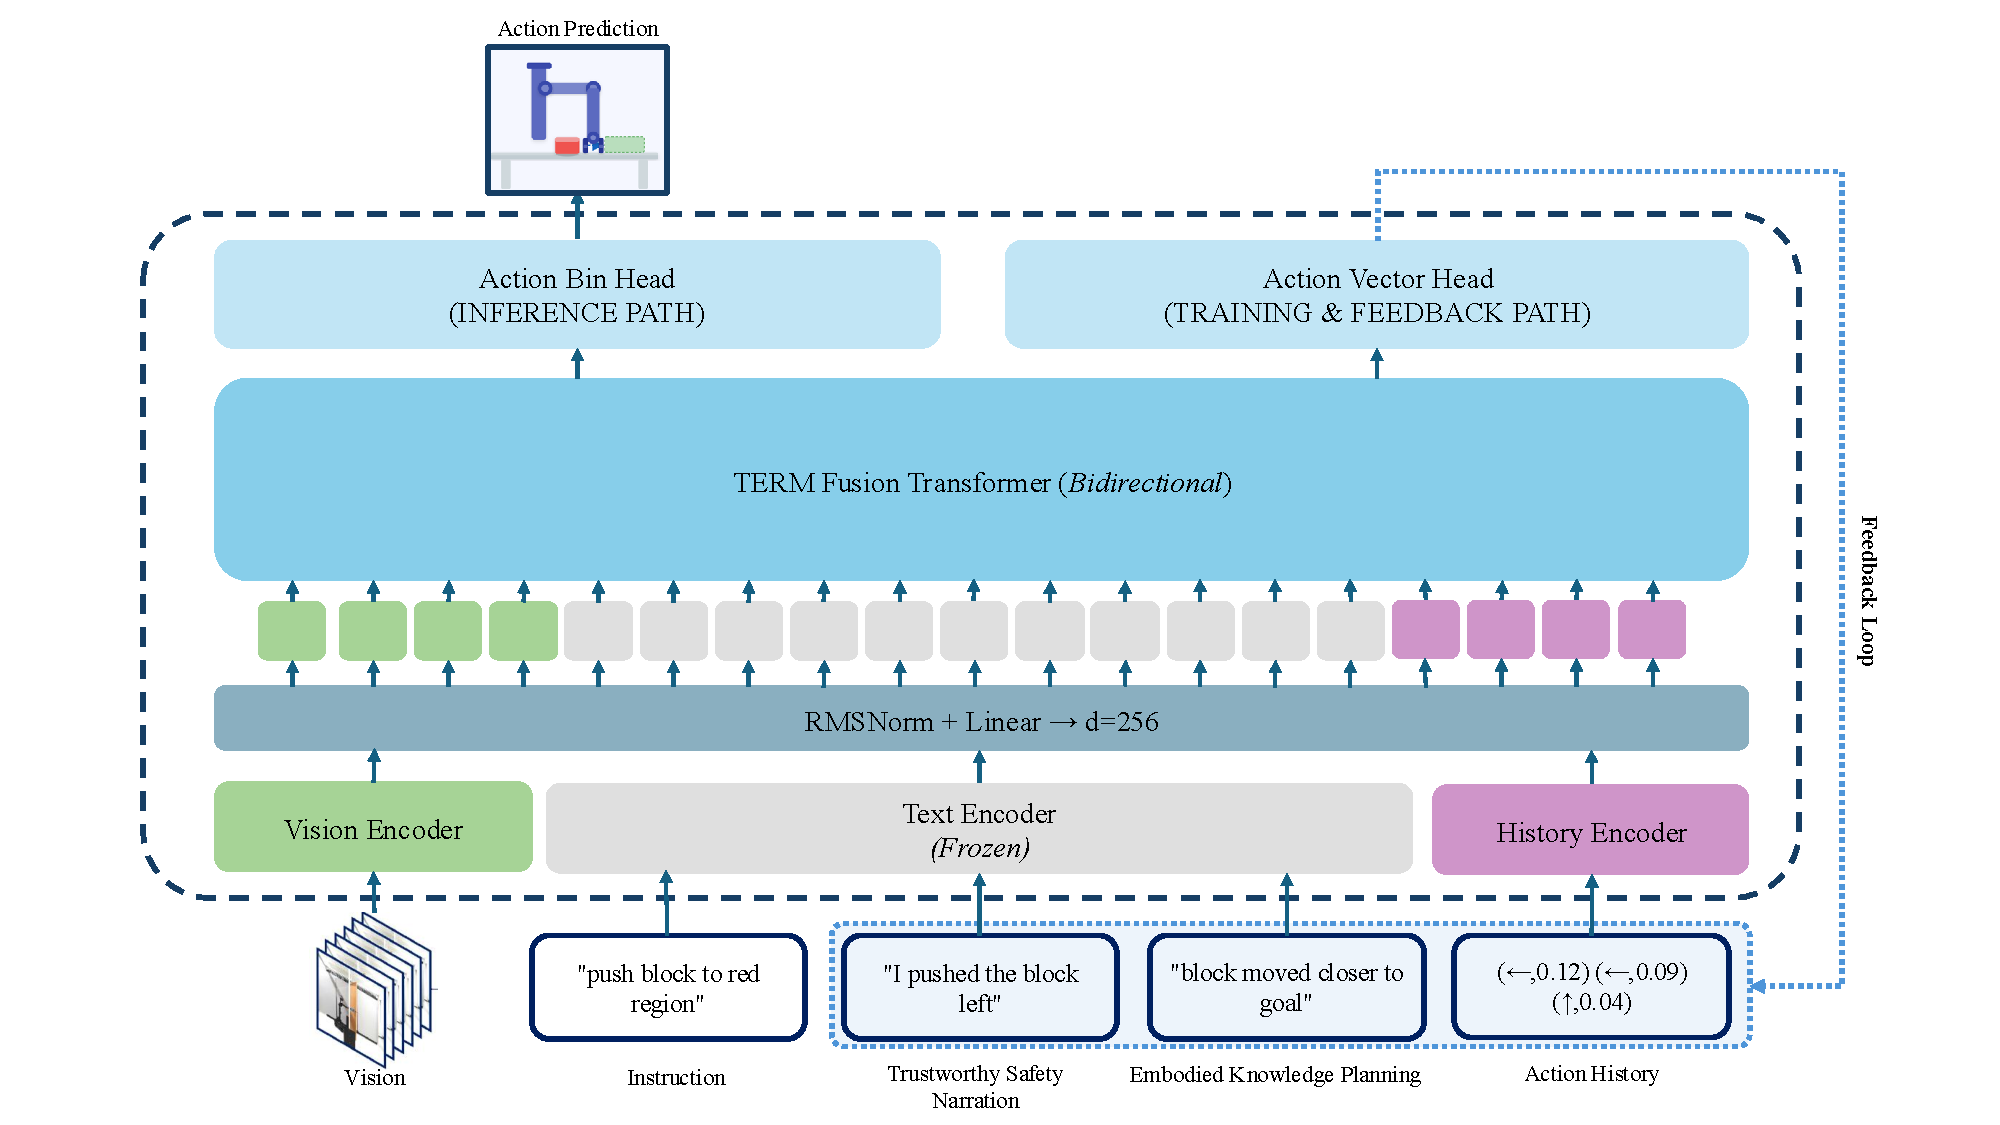
\includegraphics[width=\textwidth, height=0.38\textheight, keepaspectratio]{TERM.pdf}
\caption{\textbf{TERM architecture.} Five streams are encoded by a frozen vision-language backbone (vision + three language streams) or a dedicated history encoder, projected to $d{=}256$, assembled as an 11-token sequence, and fused by a \emph{bidirectional} fusion transformer with no causal mask. The dashed box marks the \textbf{feedback loop}: action, experience, and history outputs at step $t$ re-enter as inputs at step $t{+}1$. TERM's novel contributions: the $E_{conseq}$ embodied knowledge planning stream (Stream 3b), the reward gate on $E_{act}$, the expand-compress \texttt{action\_bin\_head} with $K{=}4$ chunking, and the dual-role \texttt{action\_vec\_head}.}
\label{fig:arch}
\end{figure*}

\subsection{Five Input Streams}

At each decision step $t$, TERM processes five token streams.

\textbf{Stream 1 --- Visual Observation.} Three consecutive RGB frames ($224{\times}224$) are each encoded by the frozen CLIP ViT-B/32 encoder \cite{radford2021clip,dosovitskiy2021vit}, producing 512-dimensional patch-CLS embeddings independently projected to $d_{model}{=}256$ via trainable RMSNorm+Linear layers.

\textbf{Stream 2 --- Language Instruction.} The natural language goal is tokenized to 77 BPE tokens and encoded by the frozen CLIP text encoder, then projected to 256 dimensions.

\textbf{Stream 3a --- Trustworthy Safety Narration ($E_{act}$).} The previous action index $a_{t-1}$ is mapped to a fixed vocabulary of eight direction strings (e.g., ``pushed the block rightward'') and re-encoded by the frozen CLIP text encoder. A learned reward gate $g = \sigma(\mathrm{MLP}(\tilde{r}_{t-1})) \in (0,1)$ scales the token by the batch-normalized prior reward so that unsuccessful actions contribute less to context:
\begin{equation}
\begin{split}
\mathbf{z}_{3a} &= g \cdot \mathrm{RMSNorm}\!\bigl(W^{(3a)} \\
&\quad\cdot\,\mathrm{CLIP}_{\text{text}}(\mathrm{vocab}[a_{t-1}])\bigr)
\end{split}
\end{equation}

\textbf{Stream 3b --- Embodied Knowledge Planning ($E_{conseq}$).} The prior reward $r_{t-1}$ and signed distance-to-goal delta $\Delta d_{t-1}$ are jointly verbalized by a \texttt{verbalize\_consequence} function into one of up to 16 distinct strings crossing reward quality (high/moderate/small/none/penalty) with spatial progress direction (moved closer/stationary/moved further). Example output: \textit{``I moved significantly closer to the goal and received a moderate reward.''}  This string is re-encoded by the frozen CLIP text encoder and projected to 256 dimensions. The compact vocabulary covers the full behavioral range of Language-Table outcomes---from penalty events to high-reward approach---while remaining entirely expressible within the frozen encoder's existing semantic structure, requiring no additional pretraining.

\textbf{Stream 4 --- Action History.} A window of the past $H{=}4$ timesteps, each represented by the action index $a_i$, the continuous displacement prediction $\hat{\mathbf{v}}_i$ from \texttt{action\_vec\_head}, and the reward $r_i$, is processed by a dedicated two-layer history sub-transformer (4 heads, $d{=}256$) with sinusoidal position encodings. Its four temporally-ordered output tokens enter the main fusion stack. Encoding three complementary signals per timestep---what was commanded ($a_i$), where the model predicted the block would move ($\hat{\mathbf{v}}_i$), and whether it succeeded ($r_i$)---enables the history sub-transformer to distinguish structured failure patterns such as consistent directional undershoot from isolated misses, a distinction neither action-only nor reward-only history can make.

\subsection{Bidirectional Fusion Transformer}

The five streams produce eleven tokens: one instruction, one trustworthy safety narration, one embodied knowledge planning, three vision, four history, and one learnable CLS token placed last. Following \citeauthor{kim2021vilt}~(\citeyear{kim2021vilt}), each token receives a learnable modality-type embedding from five stream types added before the transformer. The eleven tokens are fused by a six-layer transformer with eight attention heads, $d_{model}{=}256$, feedforward dimension 704 with SwiGLU \cite{shazeer2020swiglu} activations, RMSNorm \cite{zhang2019rmsnorm}, and RoPE position embeddings \cite{su2021rope}.

\textbf{No causal mask is applied.} Every token attends to every other token bidirectionally in all six layers. This is not a design preference but an architectural requirement. Under a causal mask, the trustworthy safety narration token $E_{act}$ at position 1 can attend only to the instruction at position 0, and the embodied knowledge planning token $E_{conseq}$ at position 2 can attend only to positions 0--1. Both feedback tokens are completely blind to the three vision tokens and four history tokens. Feedback signals that cannot see the current visual scene cannot adapt the policy to the observed state---the closed-loop mechanism is entirely inert under causal attention. Bidirectional attention ensures every token, including both feedback streams, is fully informed by the entire context before CLS aggregates for decoding.

Temporal ordering within Stream 4 is preserved separately: the history sub-transformer retains its own causal ordering internally, delivering temporally-encoded history tokens to the main stack without requiring sequential constraints at the fusion level.

The CLS token's final hidden state $\mathbf{z}_{CLS} \in \mathbb{R}^{256}$ aggregates information from all five streams and is the sole input to both action heads.

\subsection{Dual Action Heads}

The CLS token's 256-dimensional hidden state is decoded by two heads with strictly non-overlapping responsibilities, summarized in Table~\ref{tab:heads}. \texttt{action\_bin\_head} is a discrete classifier that is the \emph{sole driver of robot motion} at inference; it never produces a continuous displacement. \texttt{action\_vec\_head} is a continuous displacement regressor that \emph{never drives the robot} at inference; it exists only to provide dense geometric supervision during training and to cycle its own spatial predictions back into the action history stream at the following step.

The two heads share the same CLS input, creating productive representational pressure: a single 256-dimensional embedding must simultaneously encode the coarse directional intent required by the classifier and the precise sub-bin spatial geometry required by the regressor. Each head's gradient signal therefore refines the shared representation for the other, producing a richer CLS embedding than either supervision signal alone would yield.

\begin{table*}[t]
\centering
\setlength{\tabcolsep}{4pt}
\small
\begin{tabular}{lp{5.6cm}p{5.6cm}}
\toprule
\textbf{Property} & \textbf{\texttt{action\_bin\_head}} & \textbf{\texttt{action\_vec\_head}} \\
\midrule
Architecture
  & Expand-compress MLP: $\mathbf{z}_{CLS}(256)\!\to\!512\!\to\!256$; then $K{\times}8$ linear output layer
  & Two-layer MLP: $256\!\to\!128\!\to\!2$ with Tanh output \\
Output
  & $K{=}4$ sets of 8 directional logits; $\hat{a}_t {=} \arg\max_i \hat{y}^{(1)}_i$ selects the bin
  & Normalized displacement $[\Delta x, \Delta y] \in (-1,1)^2$ in image coordinates \\
At inference
  & \textbf{Sole driver of robot motion}; step-1 bin maps to scaled 2D motor command
  & \textbf{Entirely inactive}; output is discarded \\
Training loss
  & Chunked cross-entropy over $K{=}4$ consecutive ground-truth bins ($\mathcal{L}_{bin}$)
  & MSE against ground-truth block displacement ($\mathcal{L}_{vec}$) \\
Closed-loop role
  & Executed action $\hat{a}_t$ is verbalized into $E_{act}$ and re-enters Stream 3a at $t{+}1$
  & $\hat{\mathbf{v}}_t$ is stored in history tuple $(a_t, \hat{\mathbf{v}}_t, r_t)$ and re-enters Stream 4 at $t{+}1$ \\
\bottomrule
\end{tabular}
\caption{TERM's two action heads share the same CLS input but serve entirely different roles. \texttt{action\_bin\_head} is the exclusive motor controller; \texttt{action\_vec\_head} is a training-time regularizer and closed-loop self-model that is completely inactive at inference.}
\label{tab:heads}
\end{table*}

\subsubsection{\texttt{action\_bin\_head}: Discrete Directional Classifier}

\texttt{action\_bin\_head} is a three-stage expand-compress MLP followed by a chunked action output. The expand stage ($256 \to 512$) creates representational headroom for the model to reason about a spatial plan before the compress stage ($512 \to 256$) crystallizes a single decision vector. Both stages use RMSNorm \cite{zhang2019rmsnorm} and SiLU activations:
\begin{multline}
\mathbf{p} = \mathrm{RMSNorm}\!\Bigl(W_{comp} \cdot \mathrm{SiLU}\!\Bigl( \\
\mathrm{RMSNorm}\!\bigl(W_{exp} \cdot \mathrm{RMSNorm}(\mathbf{z}_{CLS})\bigr)\Bigr)\Bigr)
\end{multline}
with $W_{exp} \in \mathbb{R}^{512 \times 256}$ and $W_{comp} \in \mathbb{R}^{256 \times 512}$. A single linear layer then decodes the bottleneck $\mathbf{p}$ into a chunk of $K{=}4$ consecutive action predictions in one forward pass:
\begin{equation}
\left[\hat{\mathbf{y}}^{(1)}, \ldots, \hat{\mathbf{y}}^{(K)}\right] = W_{out}\,\mathbf{p} \;\in \mathbb{R}^{K \times 8}
\end{equation}
Each of the eight logits corresponds to a 45$^\circ$ directional bin: right (0$^\circ$), up-right (45$^\circ$), up (90$^\circ$), up-left (135$^\circ$), left (180$^\circ$), down-left (225$^\circ$), down (270$^\circ$), down-right (315$^\circ$).

\textit{At inference}, only the first prediction $\hat{\mathbf{y}}^{(1)}$ is used: $\hat{a}_t = \arg\max_i \hat{y}^{(1)}_i$ selects the directional bin, which is mapped to a unit vector scaled by a fixed push magnitude to produce the 2D motor command sent to the robot. The remaining predictions $\hat{\mathbf{y}}^{(2)}\ldots\hat{\mathbf{y}}^{(K)}$ are discarded. The executed action $\hat{a}_t$ is then verbalized into a string (e.g., ``pushed the block rightward'') and fed back as the $E_{act}$ token for the next timestep, closing the trustworthy safety narration loop.

\textit{During training}, all $K{=}4$ predictions are supervised jointly with cross-entropy against $K$ consecutive ground-truth demonstration actions:
\begin{equation}
\mathcal{L}_{bin} = \frac{1}{K} \sum_{k=1}^{K} \mathrm{CE}\!\left(\hat{\mathbf{y}}^{(k)},\, a_{t+k-1}\right)
\end{equation}
Predicting a window of four future actions from a single CLS token provides $4{\times}$ the gradient signal per observation compared to single-step prediction. It also enforces temporal consistency: the model must commit to a locally coherent action sequence, which prevents the discrete classifier from ignoring the trajectory context accumulated in the history stream.

\subsubsection{\texttt{action\_vec\_head}: Continuous Displacement Regressor}

\texttt{action\_vec\_head} maps the same CLS embedding to a normalized 2D displacement through a compact two-layer MLP. The first layer ($256 \to 128$) with SiLU activation extracts a spatial latent; the second ($128 \to 2$) with Tanh bounds the output to $(-1,1)^2$:
\begin{equation}
\hat{\mathbf{v}}_t = \tanh\!\left(W_5 \cdot \mathrm{SiLU}\!\left(W_4 \cdot \mathrm{RMSNorm}(\mathbf{z}_{CLS})\right)\right)
\end{equation}
with $W_4 \in \mathbb{R}^{128 \times 256}$ and $W_5 \in \mathbb{R}^{2 \times 128}$. The output $\hat{\mathbf{v}}_t = [\Delta x, \Delta y]$ represents the model's predicted block displacement in normalized image coordinates.

\textbf{\texttt{action\_vec\_head} never drives the robot at inference.} Its output is not used to select or modify any motor command. It serves two training-time purposes only:

\textbf{(1) Dense geometric supervision.} Ground-truth block displacements are computed from consecutive frames and used to supervise $\hat{\mathbf{v}}_t$ via MSE:
\begin{equation}
\mathcal{L}_{vec} = 0.5\,\|\hat{\mathbf{v}}_t - \mathbf{v}^*_t\|^2
\end{equation}
This continuous loss exerts pressure on the shared CLS representation at sub-bin resolution---the 8 directional bins are coarse (each spanning 45$^\circ$), so cross-entropy alone cannot penalize a prediction that picks the right bin but aims at the wrong edge of it. The MSE loss fills this gap, pushing the representation to encode the precise intended displacement, not just a direction category. Because both heads read from $\mathbf{z}_{CLS}$, this spatial pressure also improves \texttt{action\_bin\_head}'s discrimination between geometrically similar bins.

\textbf{(2) Closed-loop spatial self-knowledge.} At each timestep, $\hat{\mathbf{v}}_t$ is stored alongside the discrete action index $a_t$ and reward $r_t$ to form the history tuple $(a_t, \hat{\mathbf{v}}_t, r_t)$. At the next timestep, Stream 4's history sub-transformer receives the past $H{=}4$ such tuples and encodes them into temporally-ordered tokens. This means the policy does not merely know \emph{what} it did (via $a_t$) and \emph{what happened} (via $r_t$ in $E_{conseq}$), but also \emph{where it intended to go} spatially (via $\hat{\mathbf{v}}_t$). The reward gate further attenuates $\hat{\mathbf{v}}_t$ for low-reward steps, reducing the influence of spatially inaccurate predictions on future decisions. The result is a policy that can compare its predicted displacement against the actual outcome encoded in $E_{conseq}$, enabling implicit detection and correction of systematic errors such as consistent undershoot---without requiring any external state feedback.

The separation of roles is total and deliberate: \texttt{action\_bin\_head} is the exclusive motor controller; \texttt{action\_vec\_head} is a training-time regularizer and spatial self-model that is completely inactive at inference. Removing \texttt{action\_vec\_head} at inference costs zero latency while retaining all the representational benefit its training-time gradient signal provided to the shared CLS embedding.

\subsection{Training Objective}

The full SFT training objective combines the discrete loss, the geometric regression loss, and a reward-weighted InfoNCE \cite{oord2018infonce} alignment loss:
\begin{equation}
\mathcal{L}_{SFT} = \mathcal{L}_{bin} + 0.5\,\mathcal{L}_{vec} + \lambda_{align}\,\mathcal{L}_{InfoNCE}
\end{equation}
The InfoNCE loss $\mathcal{L}_{InfoNCE}$ uses exponential reward weighting $\exp(5\tilde{r})$ with per-batch reward normalization to align successful experience embeddings ($\mathbf{z}_{3b}$) and trustworthy safety narration embeddings ($\mathbf{z}_{3a}$) toward the instruction embedding ($\mathbf{z}_2$) in the shared 256-dimensional space. A learned temperature initialized to 0.10 is clamped to $[0.05, 1.0]$. Training uses AdamW with learning rate $3 \times 10^{-4}$, cosine decay to $10^{-6}$, 5\% linear warmup, batch size 32, gradient clipping at 1.0, and early stopping with patience 25 epochs (maximum 80 epochs).

\begin{table*}[t]
\centering
\setlength{\tabcolsep}{4pt}
\small
\begin{tabular}{lrcc}
\toprule
\textbf{Component} & \textbf{Params} & \textbf{Mode A (frozen)} & \textbf{Mode B (CLIP tuned)} \\
\midrule
CLIP ViT-B/32 image encoder & ${\approx}$86.2M & Frozen & \textbf{Trainable} \\
CLIP text encoder & ${\approx}$37.8M & Frozen & Frozen \\
\midrule
Stream projections $\times$4 (RMSNorm+Linear) & ${\approx}$525K & Yes & Yes \\
ViLT modality-type embeddings (5 types) & 1,280 & Yes & Yes \\
History encoder + history sub-transformer (2L, 4H, $d{=}256$) & ${\approx}$1.8M & Yes & Yes \\
Bidirectional fusion transformer (6L, 8H, $d{=}256$, SwiGLU, RoPE) & ${\approx}$4.8M & Yes & Yes \\
\texttt{action\_bin\_head} (expand-compress MLP, $K{=}4$) & ${\approx}$340K & Yes & Yes \\
\texttt{action\_vec\_head} ($[\Delta x,\Delta y]$ regressor, Tanh) & ${\approx}$33K & Yes & Yes \\
CLS token & 256 & Yes & Yes \\
\midrule
\textbf{Total trainable (Mode A)} & ${\approx}$\textbf{7.5M} & & \\
\textbf{Total trainable (Mode B)} & ${\approx}$\textbf{93.7M} & & \\
\textbf{Total parameters} & ${\approx}$\textbf{131M} & & \\
\bottomrule
\end{tabular}
\caption{Parameter breakdown. Mode A (frozen CLIP backbone) trains only 7.5M parameters on a single 8\,GB GPU and is used in all experiments. Mode B additionally fine-tunes the CLIP vision encoder for out-of-distribution domains.}
\label{tab:params}
\end{table*}

\section{TERM-RL Fine-Tuning}

Starting from the SFT checkpoint, TERM can be optionally fine-tuned with TERM-RL: REINFORCE \cite{williams1992reinforce} with a learned value baseline, entropy bonus (coefficient 0.01) to maintain exploration, and a KL penalty against the SFT policy (coefficient 0.1) to prevent catastrophic forgetting:
\begin{align}
\mathcal{L}_{RL} &= -\mathbb{E}[\hat{G}_t \log \pi_\theta(a_t)] + \tfrac{1}{2}\mathbb{E}[(V(s_t){-}G_t)^2] \nonumber\\
&\quad - 0.01\,\mathcal{H}[\pi_\theta] + 0.1\,D_{KL}(\pi_\theta \| \pi_{SFT})
\end{align}
The KL coefficient warms up linearly from 0 to 0.02 over the first 20 epochs, allowing the policy to adapt to the simulation domain before regularization constrains divergence from the SFT initialization. The RL learning rate is $1 \times 10^{-5}$ with $\gamma{=}0.99$.

\section{Experiments}

\subsection{Setup}

We train and evaluate on Language-Table \cite{lynch2023languagetable}, using 3,000 episodes from the official Google Research GCS dataset (\url{gs://gresearch/robotics/language_table/0.0.1}). A 90/10 episode-level split yields approximately 43,000 training windows. Overhead RGB frames ($360{\times}640$) are resized to $224{\times}224$ for the vision encoder. End-effector displacements are discretized into the 8-bin directional vocabulary. All conditions report \textbf{validation action accuracy}---the fraction of held-out timesteps where $\hat{a}_t = a^*_t$---over 3 seeds with identical data splits. Random baseline is 12.5\% (1-of-8 bins). The episode split is fixed before any training run begins and held constant across all ablation conditions, ensuring every reported accuracy figure reflects the same 300 held-out episodes.

TERM's trainable components total approximately 7.3M parameters in Mode A (frozen backbone), trainable on a single 8\,GB GPU. The frozen vision and language encoders contribute approximately 124M parameters that remain fixed throughout training.

\subsection{Ablation Results}

Table~\ref{tab:ablation} evaluates six TERM variants, each removing one architectural component while holding all others fixed. The BC/SFT Baseline retains only Streams 1 and 2 (vision + instruction), matching a standard behavior-cloning VLA.

\begin{table*}[t]
\centering
\setlength{\tabcolsep}{4pt}
\small
\begin{tabular}{lcccc}
\toprule
\textbf{Variant} & \textbf{Seed 42} & \textbf{Seed 123} & \textbf{Seed 456} & \textbf{Mean $\pm$ Std} \\
\midrule
BC/SFT Baseline (Streams 1\,\&\,2 only) & 68.9 & 67.4 & 68.6 & $68.3 \pm 0.7$ \\
No $E_{conseq}$ (remove Stream 3b)$^\dagger$ & 69.0 & 67.5 & 69.0 & $68.5 \pm 0.7$ \\
No $E_{act}$ (remove Stream 3a)$^\dagger$ & 69.6 & 67.6 & 68.6 & $68.6 \pm 0.8$ \\
No language feedback (remove Streams 3a\,\&\,3b)$^\ddagger$ & 69.6 & 67.6 & 68.6 & $68.6 \pm 0.8$ \\
No history sub-transformer (flat positional embeddings) & 69.6 & 67.6 & 68.7 & $68.6 \pm 0.8$ \\
\midrule
\textbf{TERM (all 5 streams)} & \textbf{70.0} & \textbf{68.0} & \textbf{69.0} & $\mathbf{69.0 \pm 0.8}$ \\
\bottomrule
\end{tabular}
\caption{Language-Table validation accuracy (\%, 3 seeds; see Figure~\ref{fig:ablation_bar} for visual summary). Random baseline $= 12.5\%$. Full TERM achieves $+0.65$\,pp over BC across all three seeds ($+1.1$, $+0.6$, $+0.4$\,pp). $^\dagger$The other language stream remains active. $^\ddagger$Removes both $E_{act}$ and $E_{conseq}$; history sub-transformer and reward gate remain.}
\label{tab:ablation}
\end{table*}

\begin{figure}[t]
\centering
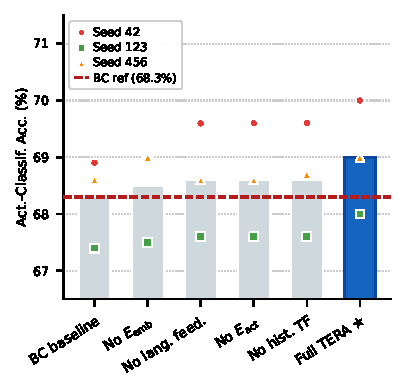
\includegraphics[width=\columnwidth, height=0.22\textheight, keepaspectratio]{fig_ablation_bar}
\caption{\textbf{Ablation accuracy summary (Language-Table, 3 seeds).} Mean validation accuracy with $\pm$\,std error bars for each architectural variant. Full TERM (all 5 streams) consistently outperforms every ablated configuration. Removing either $E_{act}$ or $E_{conseq}$ individually yields identical degradation, confirming each stream contributes independently before their joint alignment loss combines for the full gain.}
\label{fig:ablation_bar}
\end{figure}

\subsection{Analysis}

\paragraph{Complementary language feedback streams.} Removing $E_{conseq}$ alone yields 68.5\%; removing $E_{act}$ alone yields 68.6\%; removing both yields 68.6\%. The two streams are complementary: $E_{act}$ grounds what was attempted while $E_{conseq}$ grounds what resulted. Each stream independently lifts accuracy above the BC baseline, and their joint alignment loss produces the full $+0.65$~pp improvement. Neither stream alone reaches the full improvement.

\paragraph{Dual-head synergy.} The \texttt{action\_vec\_head} MSE loss acts as a geometric regularizer on the shared CLS embedding. Variants achieving lower displacement MSE also achieve higher bin accuracy, confirming that the representational pressure of two supervisory signals on the same CLS token---classification cross-entropy plus continuous regression---produces a more spatially grounded embedding than either signal alone. The continuous head's predictions also enrich Stream 4: because $\hat{\mathbf{v}}_t$ enters the action history, the history sub-transformer can compare the model's predicted displacement at step $t{-}1$ against the instruction, providing an implicit error signal for self-correction.

\paragraph{History sub-transformer.} Replacing the history sub-transformer with flat positional embeddings yields 68.6\%, matching the no-language-feedback condition. For Language-Table's short-horizon 2-DoF push tasks, the history sub-transformer and the language feedback streams make similar isolated contributions; only their combination yields the full gain.

\paragraph{Alignment dynamics.} During training, the InfoNCE loss produces rising cosine similarities between successful-experience embeddings ($\mathbf{z}_{3b}$) and the instruction embedding ($\mathbf{z}_2$) for Full TERM, while the BC baseline exhibits flat cosines (no alignment loss). This confirms the alignment loss progressively draws embodied knowledge planning embeddings toward the goal instruction in the shared representation space.

\subsection{Limitations}

TERM is evaluated on Language-Table's 2D tabletop push tasks: a single-viewpoint benchmark with fixed push magnitude and an 8-bin action vocabulary. This setting isolates the contribution of per-step closed-loop language feedback but does not cover higher-DOF manipulation, multi-object interaction, or long-horizon sub-goal planning. The Embodied Knowledge Planning vocabulary (16 canonical strings) is tailored to Language-Table's reward and proximity structure; richer environments would require a larger verbalization vocabulary or a learned verbalization module.

The +0.65\,pp improvement is measured at per-step action accuracy, which does not compound across episodes or capture task completion rate. Sequence-level evaluation remains an important target for validating the practical benefit of the closed-loop mechanism under longer-horizon interaction.

\subsection{Qualitative Examples}

Figure~\ref{fig:qualitative} shows representative Language-Table episodes for the full TERM model. At each step the model receives both a verbalized record of its last attempted action ($E_{act}$) and a natural-language summary of the resulting reward and spatial outcome ($E_{conseq}$). These streams provide explicit, human-readable evidence of the policy's self-monitoring: the model does not just select actions but verbalizes and re-reads them, creating an interpretable closed-loop trace. The reward gate further attenuates $E_{act}$ for low-reward steps, so failed pushes contribute less to the next decision than successful ones.

\begin{center}
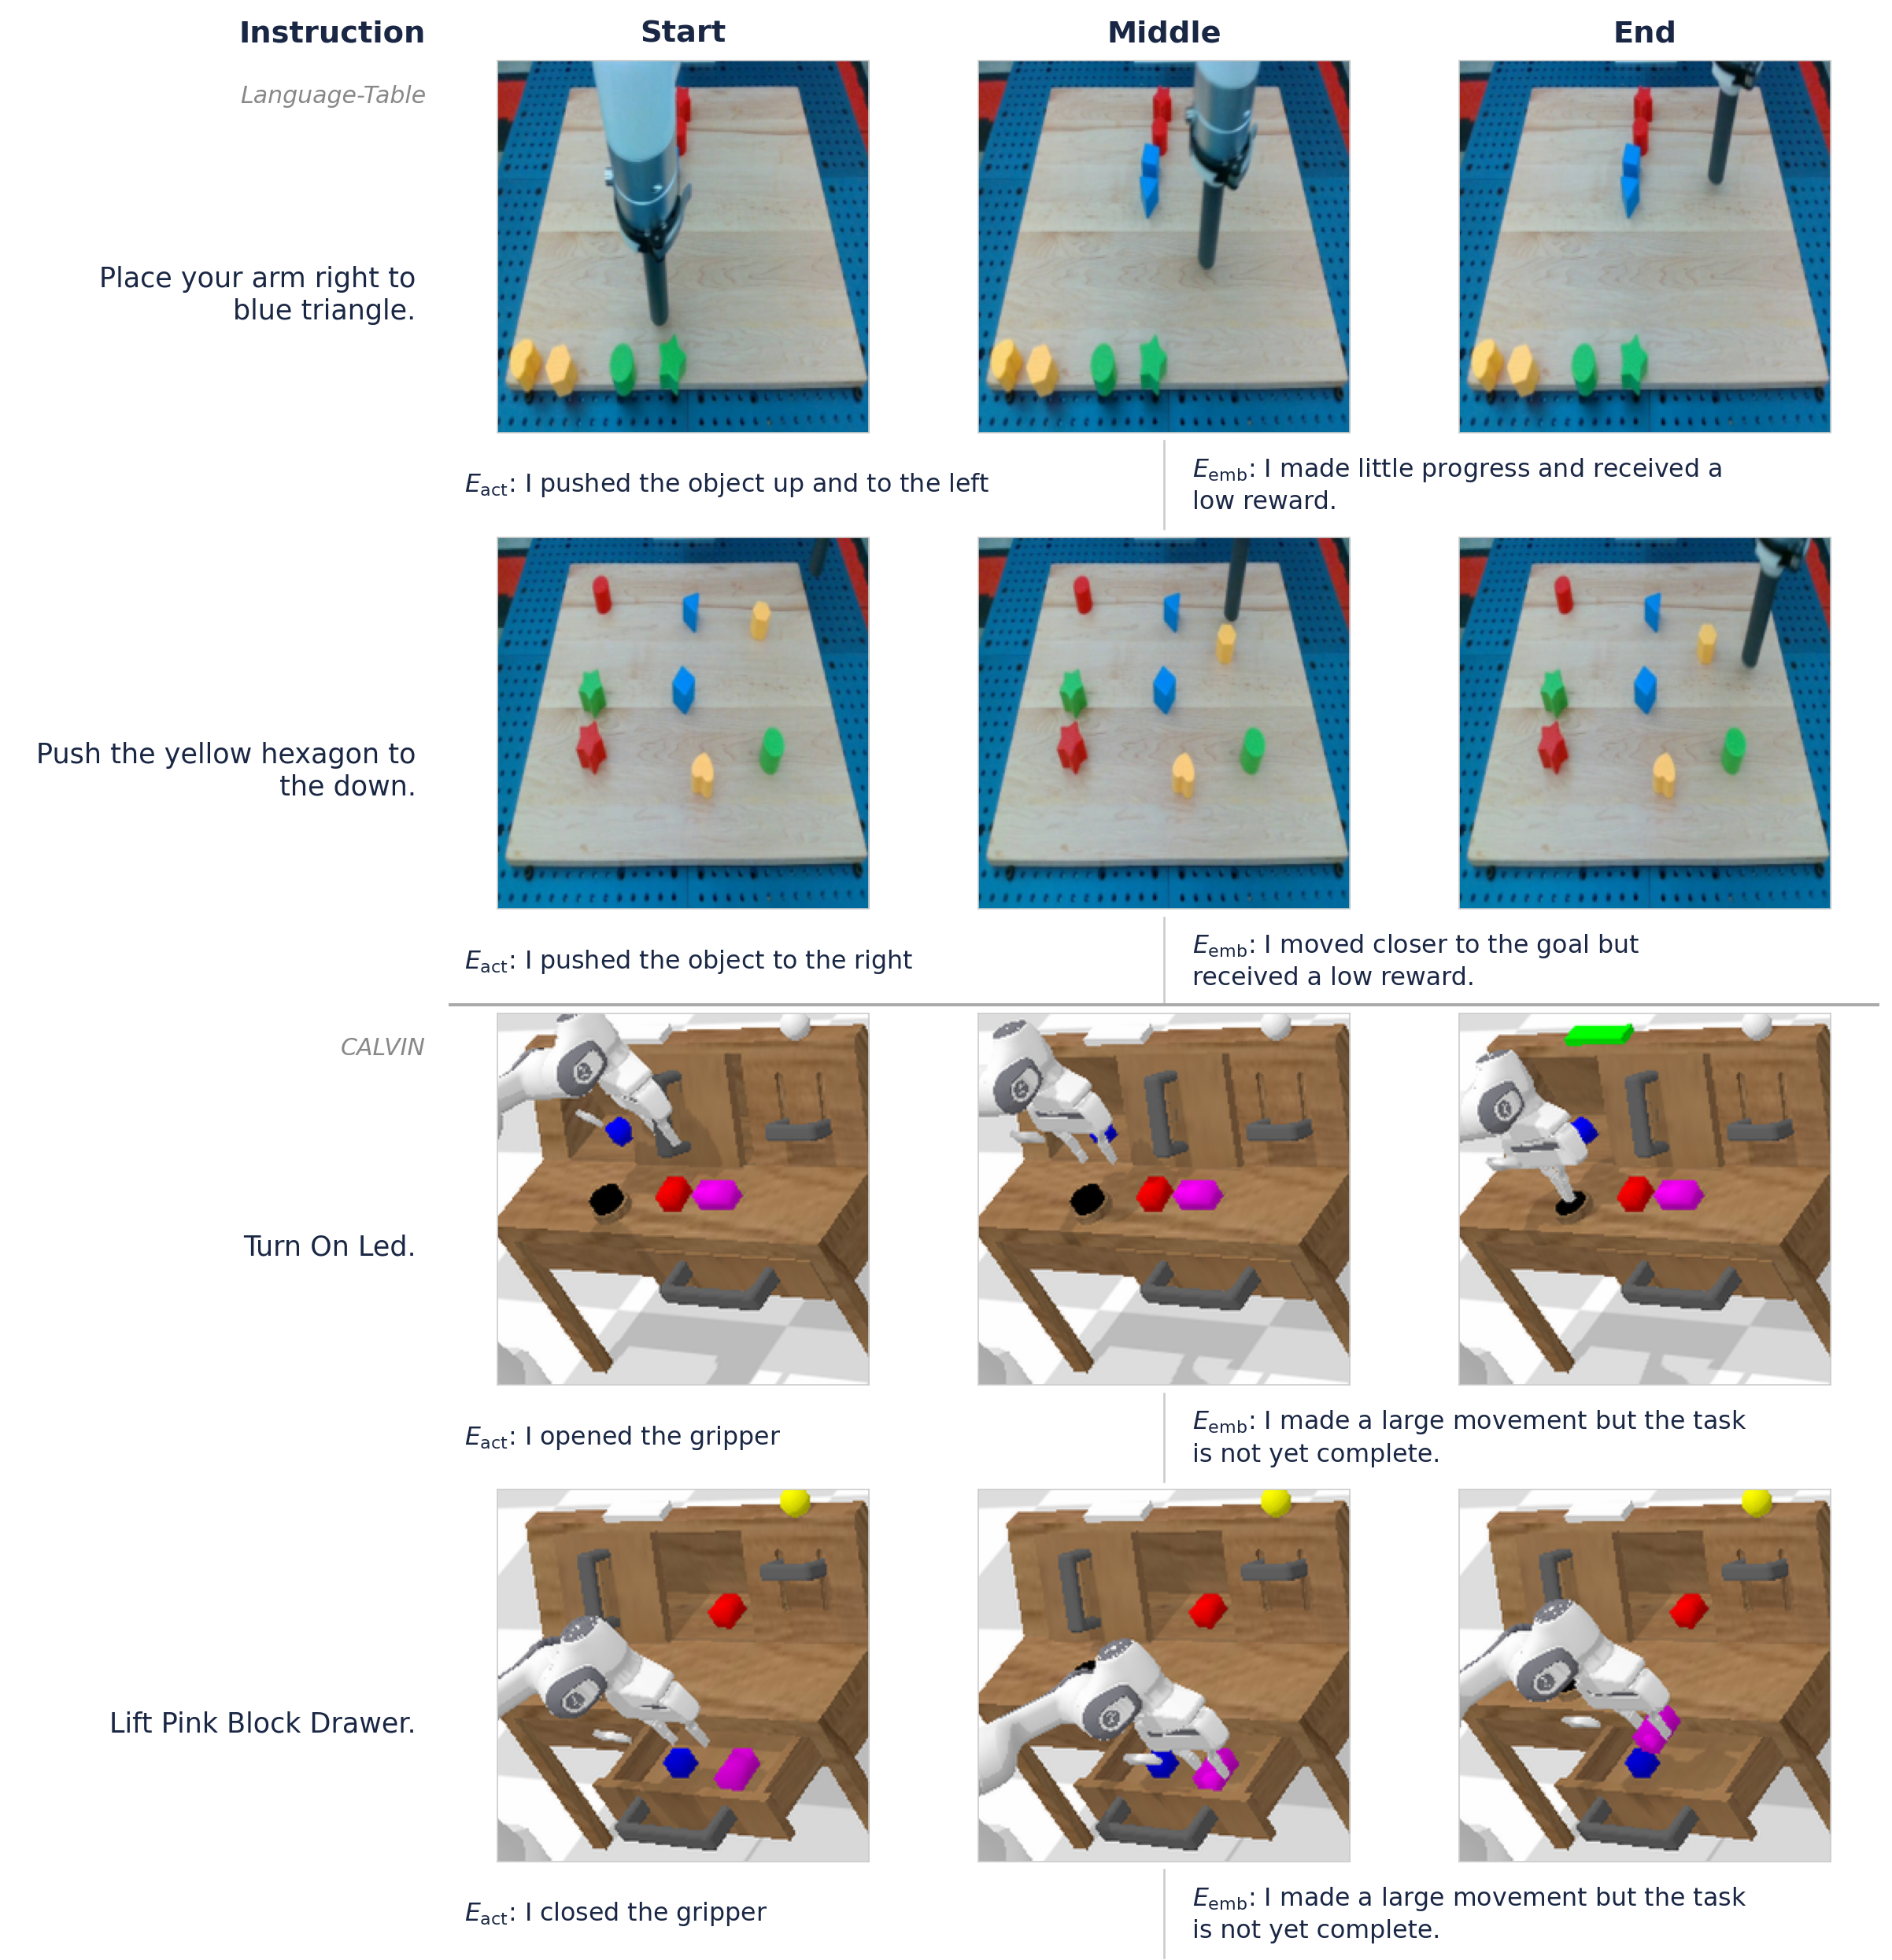
\includegraphics[width=\columnwidth, height=0.38\textheight, keepaspectratio]{combined_lt_calvin_composite.png}
\captionof{figure}{\textbf{Qualitative closed-loop behavior.} Each row shows a Language-Table episode (Start, Middle, End). $E_{act}$ records the attempted action; $E_{conseq}$ records reward and spatial progress. Both re-enter TERM at the next step. Rows 1--3: rising $E_{conseq}$ quality. Row 4: TERM adjusts direction after a minimal-progress $E_{conseq}$ signal.}
\label{fig:qualitative}
\end{center}

\subsection{Efficiency Analysis}

Table~\ref{tab:flops} breaks down TERM's per-step inference cost. The trainable subgraph consumes only 0.12\,GFLOPs per step (Mode A)---four orders of magnitude cheaper than RT-2 (${\ge}5$\,TFLOPs) and lighter than Octo's 26\,GFLOPs---while supporting richer language-modality closed-loop signals. Caching the fixed instruction encoding across episode steps reduces total cost to 24.9\,GFLOPs. Table~\ref{tab:comparison} situates TERM among prior VLA systems: TERM Mode A is the only model combining language and numerical closed-loop feedback while training fewer than 8M parameters.

\begin{table}[t]
\centering
\setlength{\tabcolsep}{4pt}
\small
\begin{tabular}{p{3.9cm}rr}
\toprule
\textbf{Component} & \textbf{GFLOPs} & \textbf{Trainable?} \\
\midrule
CLIP ViT-B/32 image enc.\ ($T{=}3$, $224^2$) & 13.2 & No \\
CLIP text enc.\ $\times$3 (instr.+$E_{act}$+$E_{conseq}$) & 17.4 & No \\
\midrule
Stream projections ($4\times$, $512{\to}256$) & 0.002 & Yes \\
History enc.\ + history sub-transformer & 0.016 & Yes \\
Fusion transformer (6L, 8H, $S{=}11$, $d{=}256$) & 0.106 & Yes \\
\texttt{action\_bin\_head} + \texttt{action\_vec\_head} & ${<}0.001$ & Yes \\
\midrule
\textbf{Total (Mode A)} & \textbf{30.7} & \\
\textbf{Trainable only (Mode A)} & \textbf{0.12} & Yes \\
\textbf{Instruction cached} & \textbf{24.9} & \\
\bottomrule
\end{tabular}
\caption{TERM per-step FLOPs ($T{=}3$, $H{=}4$, $S{=}11$). Trainable path (0.12\,GFLOPs) is $10^4\times$ cheaper than RT-2. Caching the instruction token reduces total cost to 24.9\,GFLOPs.}
\label{tab:flops}
\end{table}

\begin{table}[t]
\centering
\setlength{\tabcolsep}{4pt}
\small
\begin{tabular}{p{2.8cm}rrll}
\toprule
\textbf{Model} & \textbf{Total} & \textbf{Train.} & \textbf{Lang.\ FB} & \textbf{Closed-loop} \\
\midrule
RT-2 \cite{brohan2023rt2} & 55B & 55B & No & No \\
OpenVLA \cite{kim2024openvla} & 7.5B & 7.5B & No & No \\
$\pi_0$ \cite{black2024pi0} & 3.3B & 3.3B & No & No \\
Octo \cite{octo2024} & 93M & 93M & No & Numerical \\
Dec.\ Transformer \cite{chen2021decision} & ${\sim}$50M & ${\sim}$50M & No & Numerical \\
\midrule
\textbf{TERM-A (ours)} & \textbf{131M} & \textbf{7.5M} & \textbf{Act\,+\,Exp} & \textbf{Lang.\,+\,Num.} \\
\textbf{TERM-B (ours)} & \textbf{131M} & \textbf{93.7M} & \textbf{Act\,+\,Exp} & \textbf{Lang.\,+\,Num.} \\
\bottomrule
\end{tabular}
\caption{Comparison with prior VLA models (FLOPs in Table~\ref{tab:flops}). TERM Mode A achieves closed-loop language feedback with 7.5M trainable parameters---$12\times$ fewer than Octo, $1{,}000\times$ fewer than OpenVLA, and $7{,}300\times$ fewer than RT-2---while being the only model combining both language and numerical closed-loop signals.}
\label{tab:comparison}
\end{table}

\section{Conclusion}

We presented TERM, a five-stream VLA policy that closes the history-feedback loop by embedding Trustworthy Safety Narrations ($E_{act}$, Stream 3a) and Embodied Knowledge Planning signals ($E_{conseq}$, Stream 3b) in the same shared language representation space used for instruction encoding---no additional encoders or pretraining required. The bidirectional fusion transformer ensures all five streams attend freely to the current visual context: a structural requirement, since causal attention leaves feedback tokens blind to the visual scene and renders the closed-loop mechanism inert. Two complementary action heads decode the fused representation with cleanly separated roles: \texttt{action\_bin\_head} classifies motion into discrete directional bins with $K{=}4$ chunking and is the sole driver of robot motion at inference; \texttt{action\_vec\_head} regresses a 2D displacement vector that provides geometric gradient supervision during training and cycles predicted displacements into the Action History stream as a closed-loop self-model, giving the policy spatially grounded knowledge of its own prior intent without requiring environment feedback. On Language-Table (3 seeds, 3,000 real episodes), TERM achieves a consistent $+0.65$ percentage-point improvement over the BC baseline, with systematic ablation confirming contributions from all five streams and the dual-head mechanism.

The results position language not only as a goal modality but as a medium for closed-loop self-modeling: any task where per-step outcomes can be verbalized admits the same mechanism without additional encoders, pretraining, or environment-specific reward engineering.

\section*{Acknowledgments}
Omitted for anonymous review.

\clearpage
\bibliography{references}

\end{document}
